% Created 2022-11-24 jeu. 21:09
% Intended LaTeX compiler: pdflatex
\documentclass[10pt,table,dvipsnames,compress]{beamer}
\usepackage[utf8]{inputenc}
\usepackage[T1]{fontenc}
\usepackage{graphicx}
\usepackage{longtable}
\usepackage{wrapfig}
\usepackage{rotating}
\usepackage[normalem]{ulem}
\usepackage{amsmath}
\usepackage{amssymb}
\usepackage{capt-of}
\usepackage{hyperref}
\usetheme{default}
\useinnertheme{rounded}
\useoutertheme[subsection=false]{miniframes}
\date{}
\title{Cartes de carbone forestier pour le suivi et la conservation des forêts en Nouvelle-Calédonie}
\title[CARBOFORCAL]{Cartes de carbone forestier pour le suivi et la conservation des forêts en Nouvelle-Calédonie}
\usepackage{lmodern}
\usepackage{pgf}
\usepackage{color}
\usepackage[english,french]{babel}
\definecolor{vertmoyen}{RGB}{51,110,23} % vert moyen
\definecolor{blueFRB}{HTML}{31859c}
\usecolortheme[named=blueFRB]{structure}
\usepackage{tabularx} % varier la largeur du tableau
\usepackage{layout}
\setlength{\LTleft}{-5cm plus 1 fill}
\setlength{\LTright}{-5cm plus 1 fill}
\usepackage{booktabs}
\usepackage{arydshln} %% dashlines for tabular
\newcommand{\logit}{\text{logit}}
\newcommand{\bs}[1]{\boldsymbol{#1}}
\newcommand{\R}{\textnormal{\sffamily\bfseries R}}
\newcommand{\pkg}[1]{{\fontseries{b}\selectfont #1}}
\newcolumntype{C}[1]{>{\centering\arraybackslash}m{#1}}

\setbeamertemplate{footline}[frame number]
\setbeamertemplate{frametitle}{%
\usebeamerfont{frametitle}\insertframetitle%
\vphantom{g} % To avoid fluctuations per frame
\par
\centering 
\includegraphics[width=\textwidth]{figs/Barre_couleur}
}
\beamertemplatenavigationsymbolsempty

% Logo
\newif\ifplacelogo % create a new conditional
\logo{\ifplacelogo
\includegraphics[width=0.4\textwidth]{figs/partners_logos}\fi}

%Call table of contents at the beginning of each section
\AtBeginSection[]{
\placelogotrue
\begin{frame}
\frametitle{Plan}
\begin{columns}[c]
\begin{column}{0.5\textwidth}
\tableofcontents[sections=1,currentsection]
\vspace{0.5cm}
\tableofcontents[sections=2,currentsection]
\end{column}
\begin{column}{0.5\textwidth}
\tableofcontents[sections=3,currentsection]
\vspace{0.5cm}
\tableofcontents[sections=4,currentsection]
\end{column}
\end{columns}
\end{frame}
\placelogofalse
}

\AtBeginSubsection[]{}

\hypersetup{
colorlinks=true,
linkcolor=Black,
filecolor=Maroon,
citecolor=Blue,
urlcolor=Maroon}

% Disable monospaced font for URLs
\urlstyle{same}

\hypersetup{
 pdfauthor={Ghislain Vieilledent},
 pdftitle={Cartes de carbone forestier pour le suivi et la conservation des forêts en Nouvelle-Calédonie},
 pdfkeywords={},
 pdfsubject={},
 pdfcreator={Emacs 27.1 (Org mode 9.5.3)}, 
 pdflang={English}}
\begin{document}


% Title page
{
  \setbeamertemplate{navigation symbols}{}
  \begin{frame}[plain, noframenumbering]
  \begin{center}
  \small{\textbf{CARBOFORCAL -- Nouméa -- Vendredi 25 Novembre 2022}}
  \end{center}
  \vspace{-0.5cm}
  \titlepage % Presentation first page
  \vspace{-3cm}
  \begin{center}
    
\includegraphics[width=\textwidth]{figs/Barre_couleur}
    
    \vspace{0.25cm}
    
    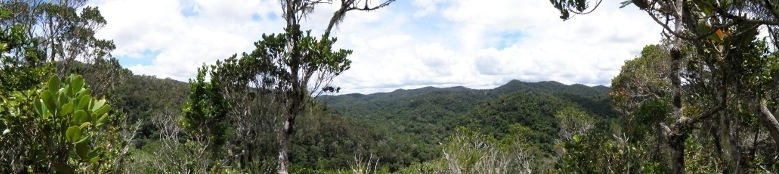
\includegraphics[width=10cm]{figs/Banniere}
    
    \small{Ghislain VIEILLEDENT$^{1, 2}$\hspace{0.25cm}Thomas IBANEZ$^{1, 2}$\hspace{0.25cm}CARBOFORCAL$^{2}$}
      
    \vspace{0.25cm}
    
    {\scriptsize
      \begin{tabular}{l}
        $[1]$ \textbf{Cirad} UMR AMAP, $[2]$ \textbf{CARBOFORCAL} UMR AMAP, Oeil, IAC
      \end{tabular}
    }

    \vspace{0.25cm}
    
    
\includegraphics[width=0.5\textwidth]{figs/partners_logos}
    
  \end{center}
  \end{frame}
}

% %%%%%%%%%%%%%%%%%%%%%%%%%%%%%%%%%%%%%%%%%%%%%%%%%%%%%%%%%%%%%%%%

\placelogotrue
\begin{frame}
  \frametitle{Plan}
  \begin{columns}[c]
    \begin{column}{0.5\textwidth}
      \tableofcontents[sections=1]
      \vspace{0.5cm}
      \tableofcontents[sections=2]
    \end{column}
    \begin{column}{0.5\textwidth}
        \tableofcontents[sections=3]
        \vspace{0.5cm}
        \tableofcontents[sections=4]
    \end{column}
  \end{columns}
\end{frame}
\placelogofalse

\section{Introduction}
\label{sec:org29993e1}

\subsection{Contexte}
\label{sec:org6c863b8}

\begin{frame}[label={sec:org6b85bd6}]{Changements climatiques dans le Pacifique}
\begin{itemize}
\item Changement climatique lié aux émissions de GES dans l'atmosphère.
\item Les communautés du Pacifique seront les premières impactées (montée des eaux).
\item Impact sur la biodiversité (Pouteau et al. 2016: 52-84\% des espèces d'arbres perdront > 50\% de leur habitat)
\end{itemize}

\begin{figure}[htbp]
\centering
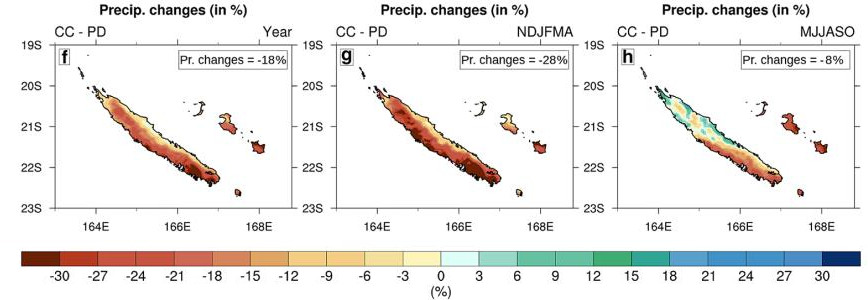
\includegraphics[width=\textwidth]{figs/Dutheil2021_cc.jpg}
\caption{Prévisions de changement de précipitations en Nouvelle Calédonie. Dutheil et al. 2021.}
\end{figure}
\end{frame}

\begin{frame}[label={sec:org8de0168}]{Déforestation en Nouvelle-Calédonie}
\begin{itemize}
\item Déforestation et dégradation des forêts: 10--20\% des émissions de GES dans l'atmospère.
\item Couvert forestier en NC: 7745 km\textsuperscript{2} en 2020 (\(\sim\) 46 \% du territoire).
\item Inclus: forêt humide, sèche, mangroves, plantations, maquis arbustif (cf. définition FAO: H > 5 m, > 10\% de couvert arboré, 0.5 ha).
\item Déforestation: 31 km\textsuperscript{2}/an sur la période 2010-2020.
\end{itemize}

\begin{figure}[htbp]
\centering
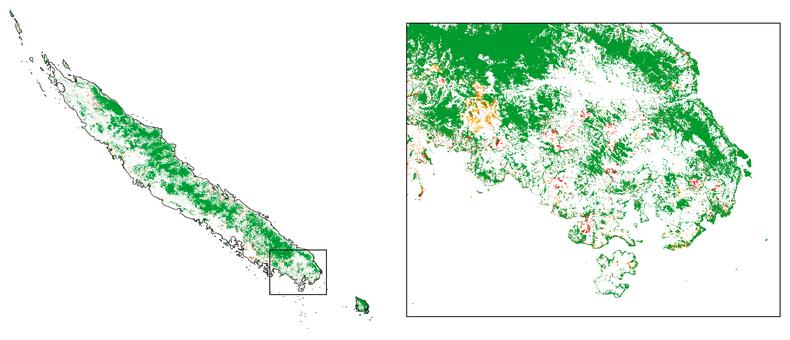
\includegraphics[width=0.8\textwidth]{figs/deforestation-NC.jpg}
\caption{Déforestation 2000--2010--2020 en Nouvelle-Calédonie. Vieilledent et al. 2022. \url{https://forestatrisk.cirad.fr/newcal}}
\end{figure}
\end{frame}

\begin{frame}[label={sec:org15399ca}]{Stock et émissions de carbone}
\begin{columns}
\begin{column}{0.6\columnwidth}
\begin{itemize}
\item Pas d'estimations précises des émissions de carbone (et CO\textsubscript{2}) associées à la déforestation.
\item Manque d'informations sur:
\begin{itemize}
\item Les stocks de carbone forestier à l'échelle de la Nouvelle-Calédonie.
\item La variation de ces stocks dans l'espace (structure et composition forestière variables).
\end{itemize}
\item Estimations ponctuelles (inventaires) des stocks de carbone en Nouvelle-Calédonie (150 t/ha \textpm{}42, Blanchard et al. 2016).
\end{itemize}
\end{column}

\begin{column}{0.4\columnwidth}
\begin{figure}[htbp]
\centering
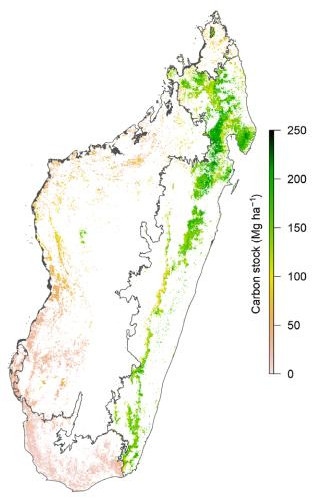
\includegraphics[width=0.85\textwidth]{figs/Cstock_Mada.jpg}
\caption{Carte des stocks de carbone forestier à Madagascar (2010). Vieilledent et al. 2016.}
\end{figure}
\end{column}
\end{columns}
\end{frame}

\subsection{Objectifs}
\label{sec:orgb85d0f6}

\begin{frame}[label={sec:org8893962}]{Objectifs}
\begin{itemize}
\item Élaborer des cartes de carbone forestier.
\item A haute résolution (\(\leq\) 100 m).
\item Avec suivi périodique dans le temps (annuel ou pluriannuel).
\end{itemize}

\begin{figure}[htbp]
\centering
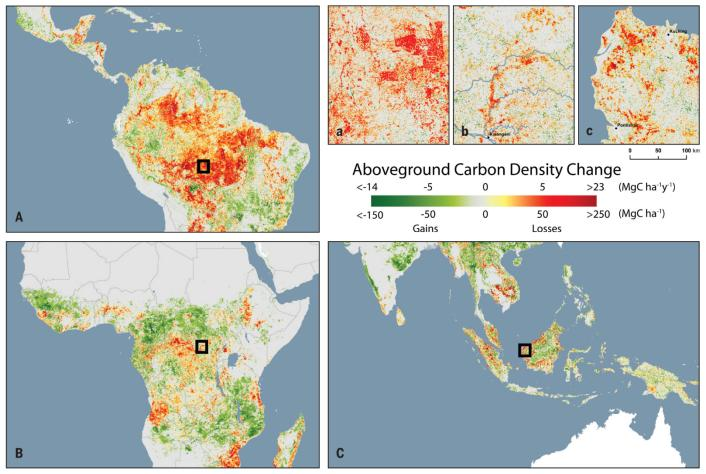
\includegraphics[width=0.7\textwidth]{figs/Baccini2017_Cchange.jpg}
\caption{Carte de changement des stocks de carbone (2004--2014). Baccini et al. 2017.}
\end{figure}
\end{frame}

\subsection{Intérêts}
\label{sec:orge15760b}

\begin{frame}[label={sec:org8cfb916}]{Intérêts des cartes de carbone forestier}
\begin{enumerate}
\item \alert{SCIENCE} \\
Rôle des forêts tropicales en Nouvelle-Calédonie dans le cycle du carbone.
\item \alert{TERRITOIRE} \\
Suivi de l'évolution du couvert forestier.
\item \alert{ECONOMIE} \\
Participation au mécanisme REDD+ et financement de projets de conservation des forêts.
\end{enumerate}
\end{frame}

\begin{frame}[label={sec:org0900691}]{Intérêts pour la SCIENCE}
Rôle des forêts tropicales en Nouvelle-Calédonie dans le cycle du carbone:

\begin{itemize}
\item Estimation des stocks de carbone forestier en NC et de leur variation dans l'espace.
\item Estimation des émissions liées à la déforestation en NC.
\end{itemize}

\vspace{0.25cm}

\begin{center}
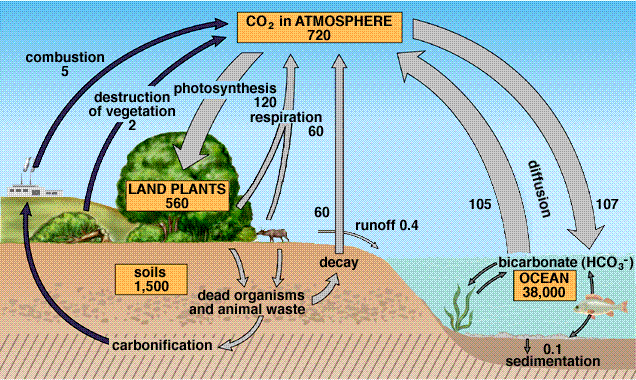
\includegraphics[width=0.6\textwidth]{figs/carbon_cycle.png}
\end{center}
\end{frame}

\begin{frame}[label={sec:org33bb818}]{Intérêts pour le TERRITOIRE}
\begin{itemize}
\item Suivi direct du changement de couvert forestier via les stocks de carbone:\\
Déforestation, Dégradation/Séquestration, Reforestation.
\item Identification des hotspots de déforestation et des zones prioritaires pour la conservation.
\item Suivi de la biodiversité et des services écosystémiques (disponibilité en eau) associés à la couverture forestière.
\end{itemize}

\vspace{0.25cm}

\begin{center}
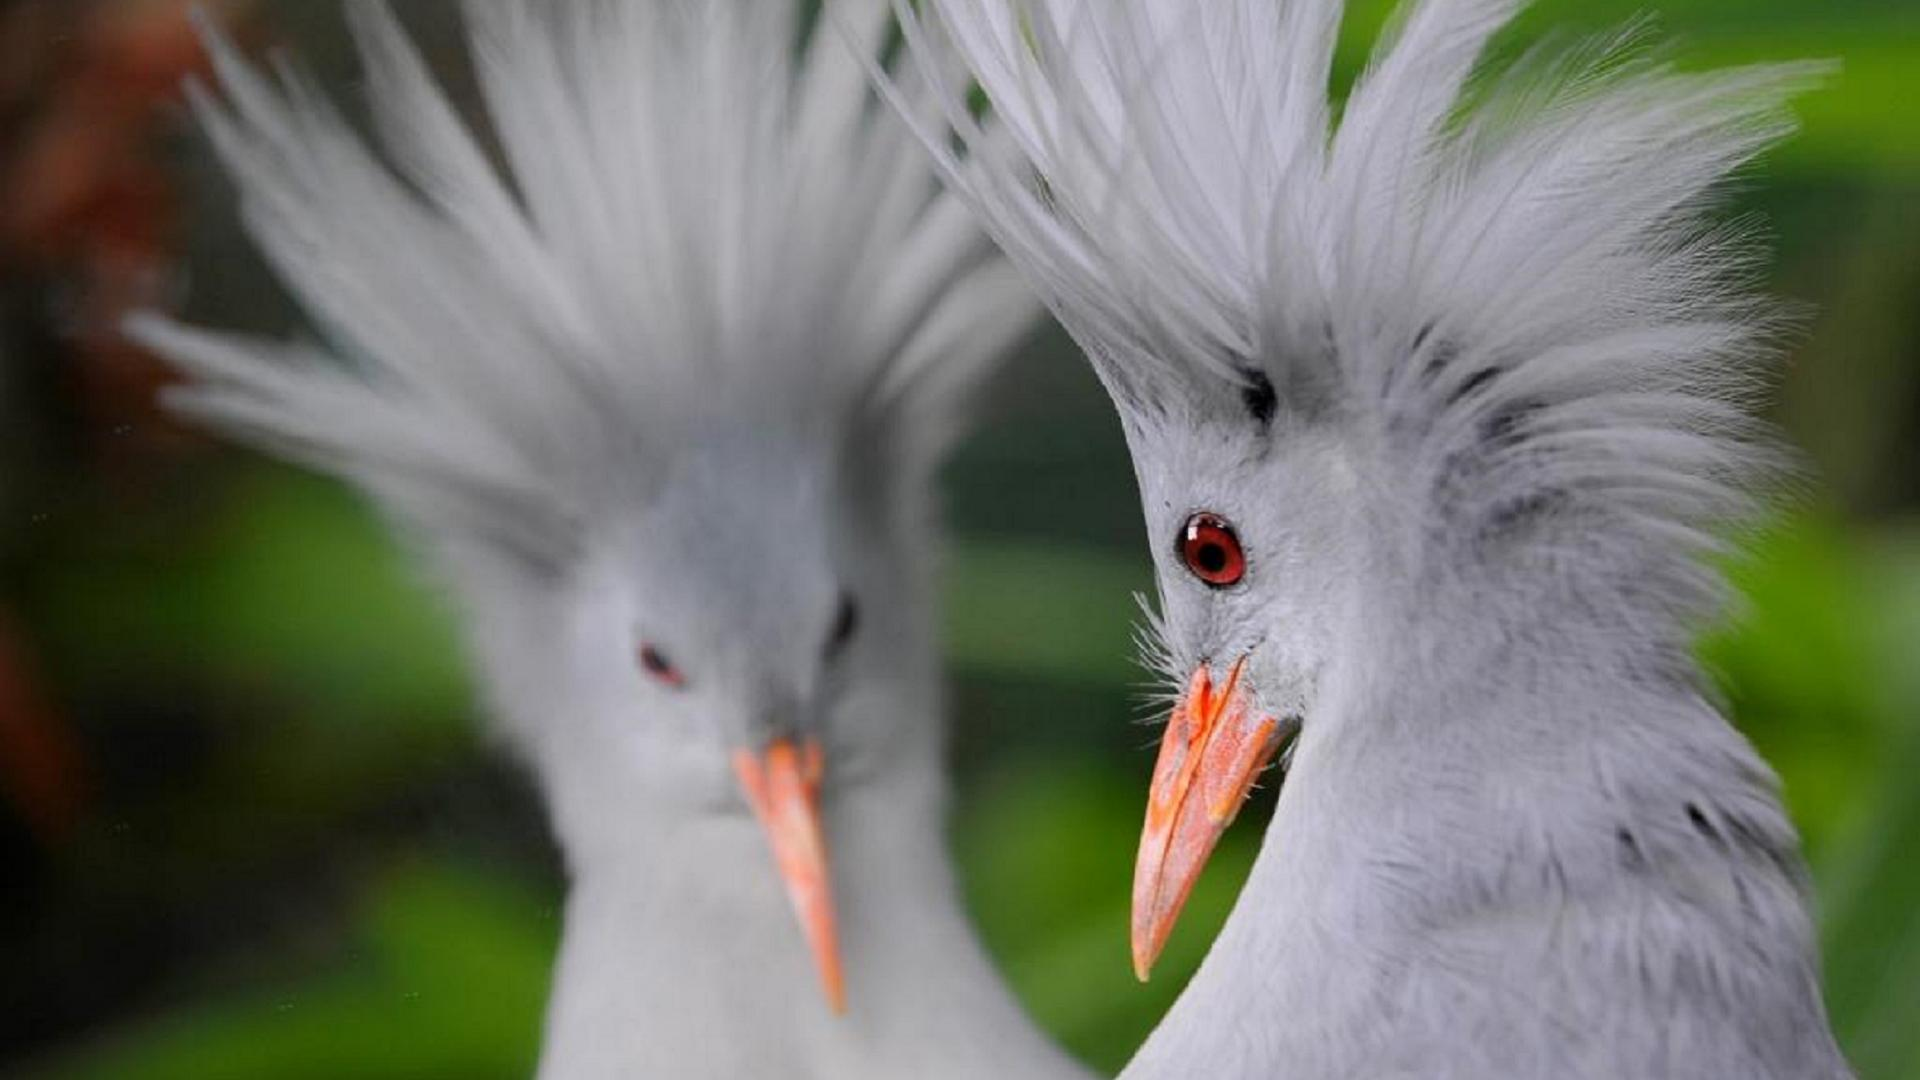
\includegraphics[height=0.3\textheight]{figs/Cagou-WWF.jpg}
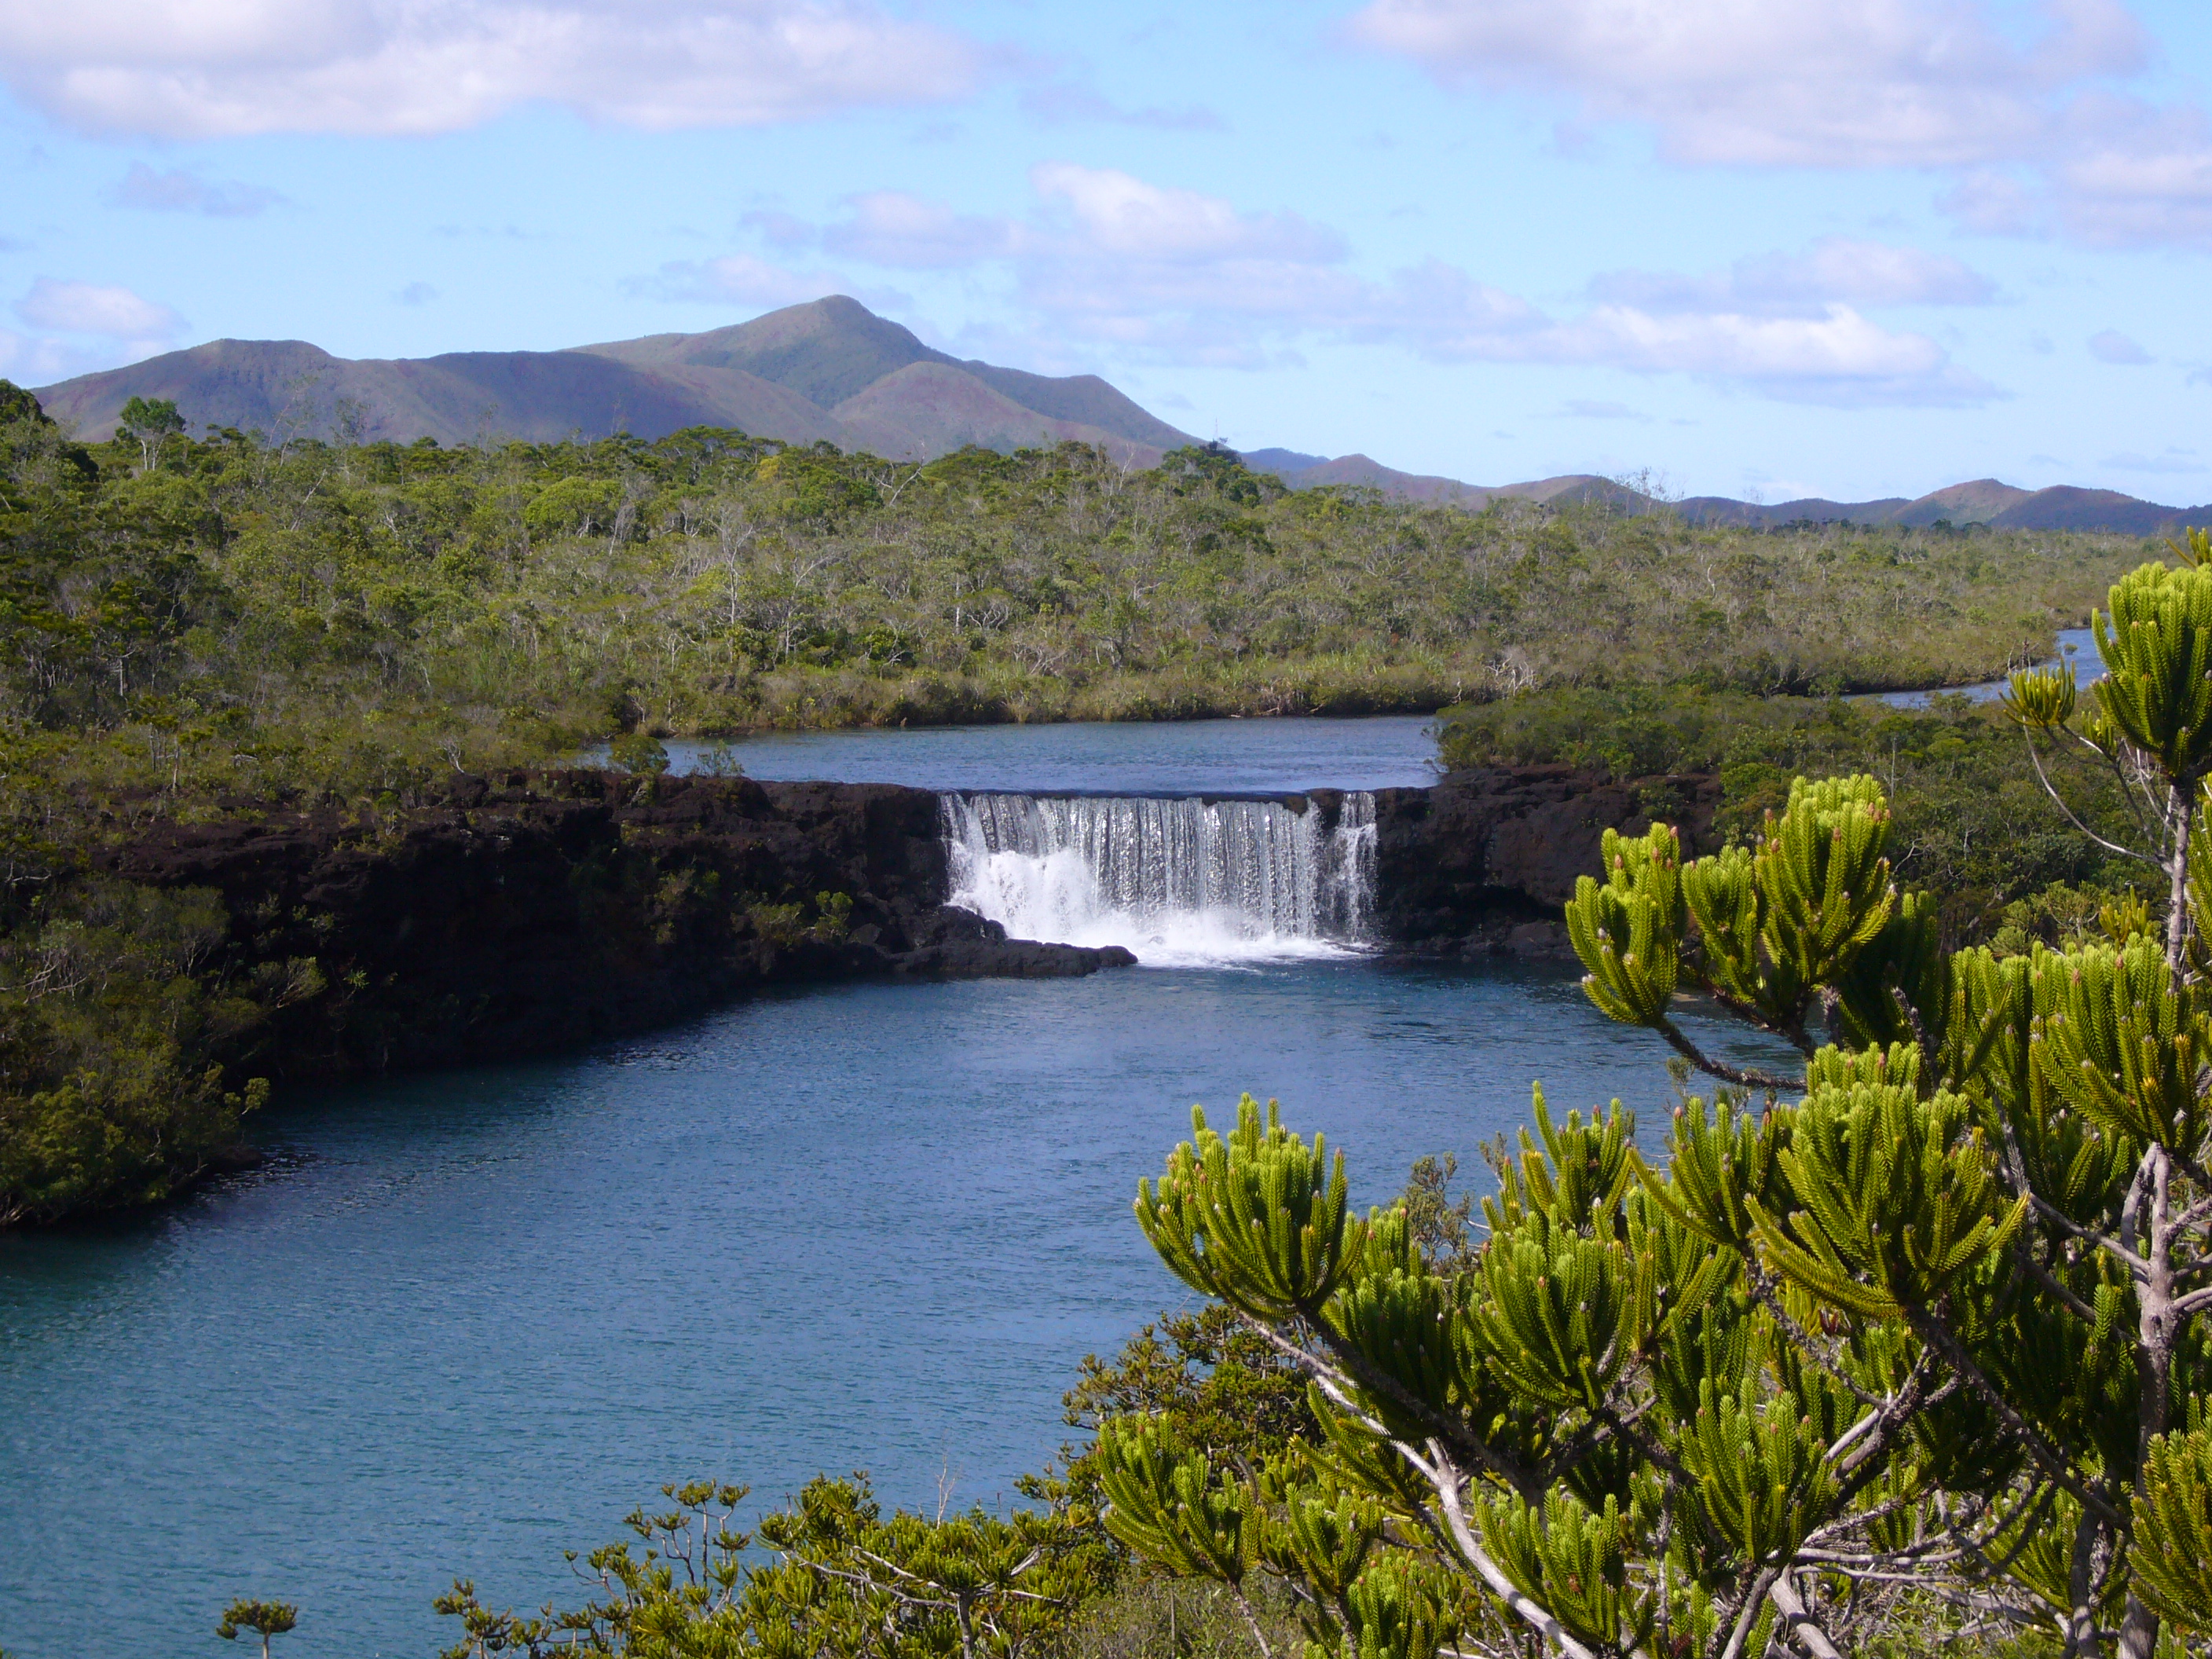
\includegraphics[height=0.3\textheight]{figs/Chutes_de_la_madeleine.JPG}
\end{center}
\end{frame}

\begin{frame}[label={sec:orgf6cc517}]{Intérêts ECONOMIQUES}
\begin{itemize}
\item Participation au mécanisme REDD+: Reducing Emissions from Deforestation and forest Degradation.
\item Les tonnes de CO\textsubscript{2} non-émises (évitées) peuvent \alert{potentiellement} être créditées.
\item Estimation à 6 \texteuro{}/t de CO\textsubscript{2} pour les projets forestiers sur le marché volontaire (en hausse constante).
\item Nouvelle-Calédonie, 3100 ha/an x 150 t/ha x 44/12 x 6 \texteuro{}/t = 10 M\texteuro{}/an.
\end{itemize}

\begin{center}
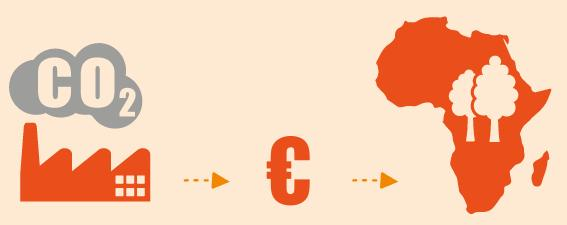
\includegraphics[width=0.4\textwidth]{figs/REDD.jpg}
\end{center}
\end{frame}

\begin{frame}[label={sec:org8f06009}]{Intérêts ECONOMIQUES}
\begin{itemize}
\item \alert{Pourrait} permettre d'attirer les investisseurs pour la conservation des forêts en Nouvelle-Calédonie.
\item Compensation des émissions liées aux activités économiques (mines et agriculture).
\item Implication accrue de la Nouvelle-Calédonie dans la lutte contre les émissions de CO\textsubscript{2} et le changement climatique.
\end{itemize}

\vspace{0.25cm}

\begin{center}
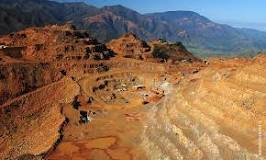
\includegraphics[height=0.3\textheight]{figs/mines.jpg}
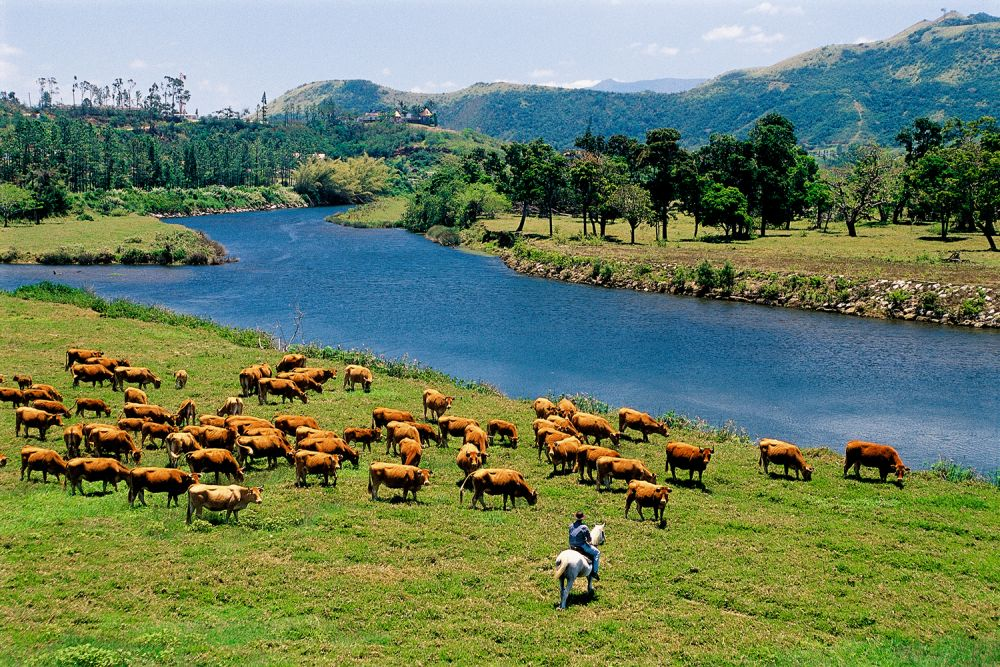
\includegraphics[height=0.3\textheight]{figs/agriculture.jpg}
\end{center}
\end{frame}


\section{Méthode}
\label{sec:orge8065df}

\subsection{Données de terrain}
\label{sec:org896aece}

\begin{frame}[label={sec:orgd10d81c}]{Données de terrain}
\begin{itemize}
\item Réseau de parcelles NC-PIPPN:\\
New Caledonian Plant Inventory and Permanent Plots Network.
\item > 500 parcelles dont 21 de 1ha, 70,000 arbres inventoriés.
\item Estimations ponctuelles des stocks de carbone (en tC/ha).
\item A compléter par d'autres parcelles, certaines permanentes.
\end{itemize}

\begin{center}
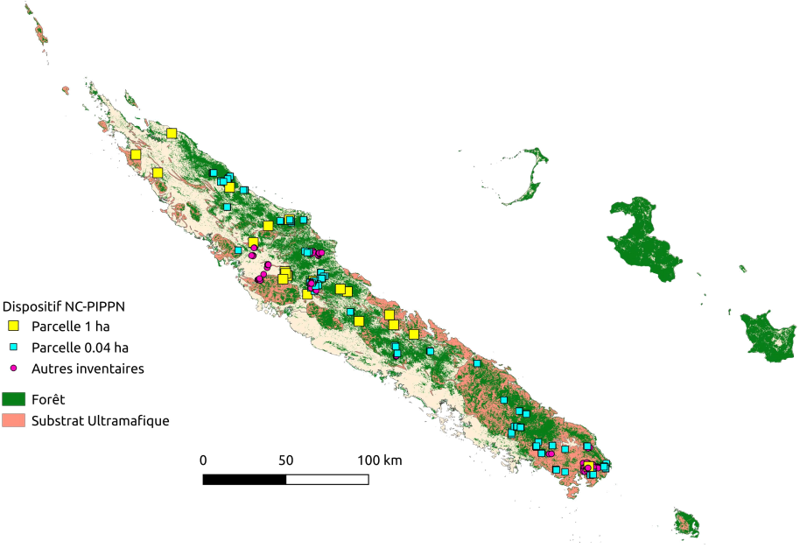
\includegraphics[width=0.7\textwidth]{figs/ncpippn-plots.png}
\end{center}
\end{frame}

\subsection{Survol drone LiDAR}
\label{sec:org50f4a96}

\begin{frame}[label={sec:orgc6ff37a}]{Survol drone LiDAR}
\begin{itemize}
\item Survol des parcelles de terrain avec un drone équipé d'un LiDAR.
\item Estimation d'une relation entre stock de carbone mesuré sur le terrain (C\textsubscript{i}) et hauteur de canopée issue du LiDAR (L\textsubscript{i}): \(C_i = \alpha L_i^{\beta}\).
\item Obtention des stocks de carbone sous les bandes LiDAR.
\item Multiplication du nombre d'observations terrain.
\end{itemize}

\begin{center}
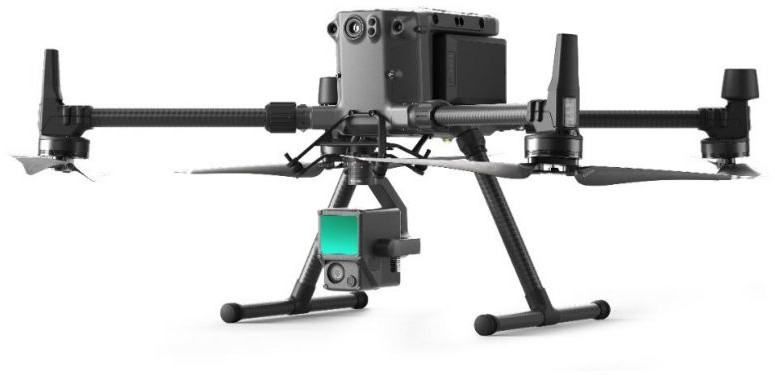
\includegraphics[width=0.3\textwidth]{figs/lidar-drone.jpg}
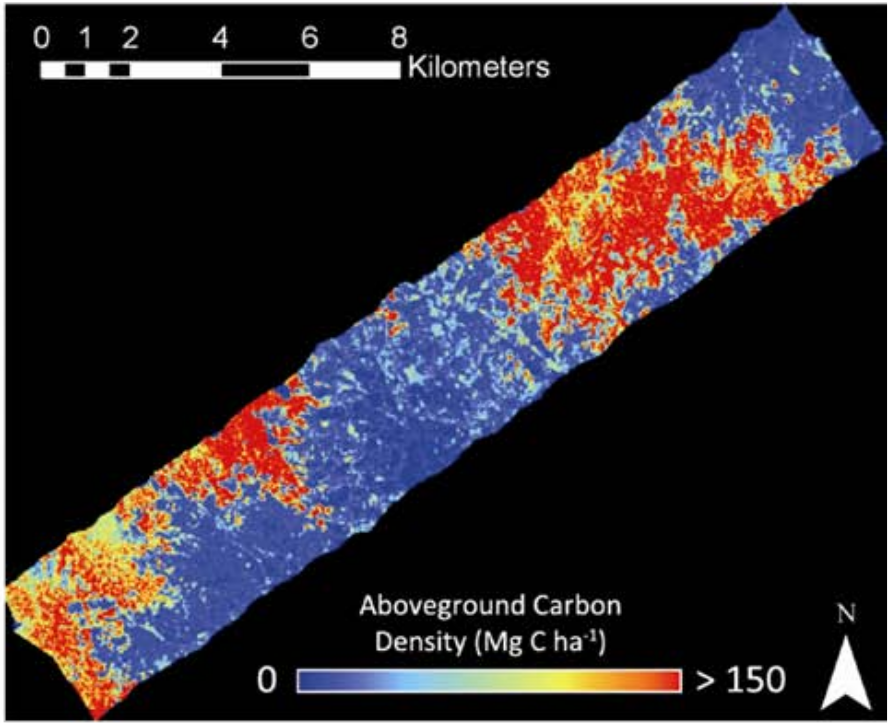
\includegraphics[width=0.4\textwidth]{figs/map-lidar.png}
\end{center}
\end{frame}

\subsection{Cartographie via images Sentinel-2}
\label{sec:orge5bae9a}

\begin{frame}[label={sec:org66b2767}]{Cartographie via images Sentinel-2}
\begin{itemize}
\item Utilisation des images Sentinel-2 pour l'extrapolation des stocks à l'ensemble du territoire.
\item Calibration d'un modèle \(C_i=f(S_i)\) où S\textsubscript{i} représente l'information spectrale issue des images Sentinel-2 pour le pixel \(i\).
\item Mise à jour périodique des prédictions grace aux acquisitions régulières des images Sentinel-2.
\end{itemize}

\begin{figure}[htbp]
\centering
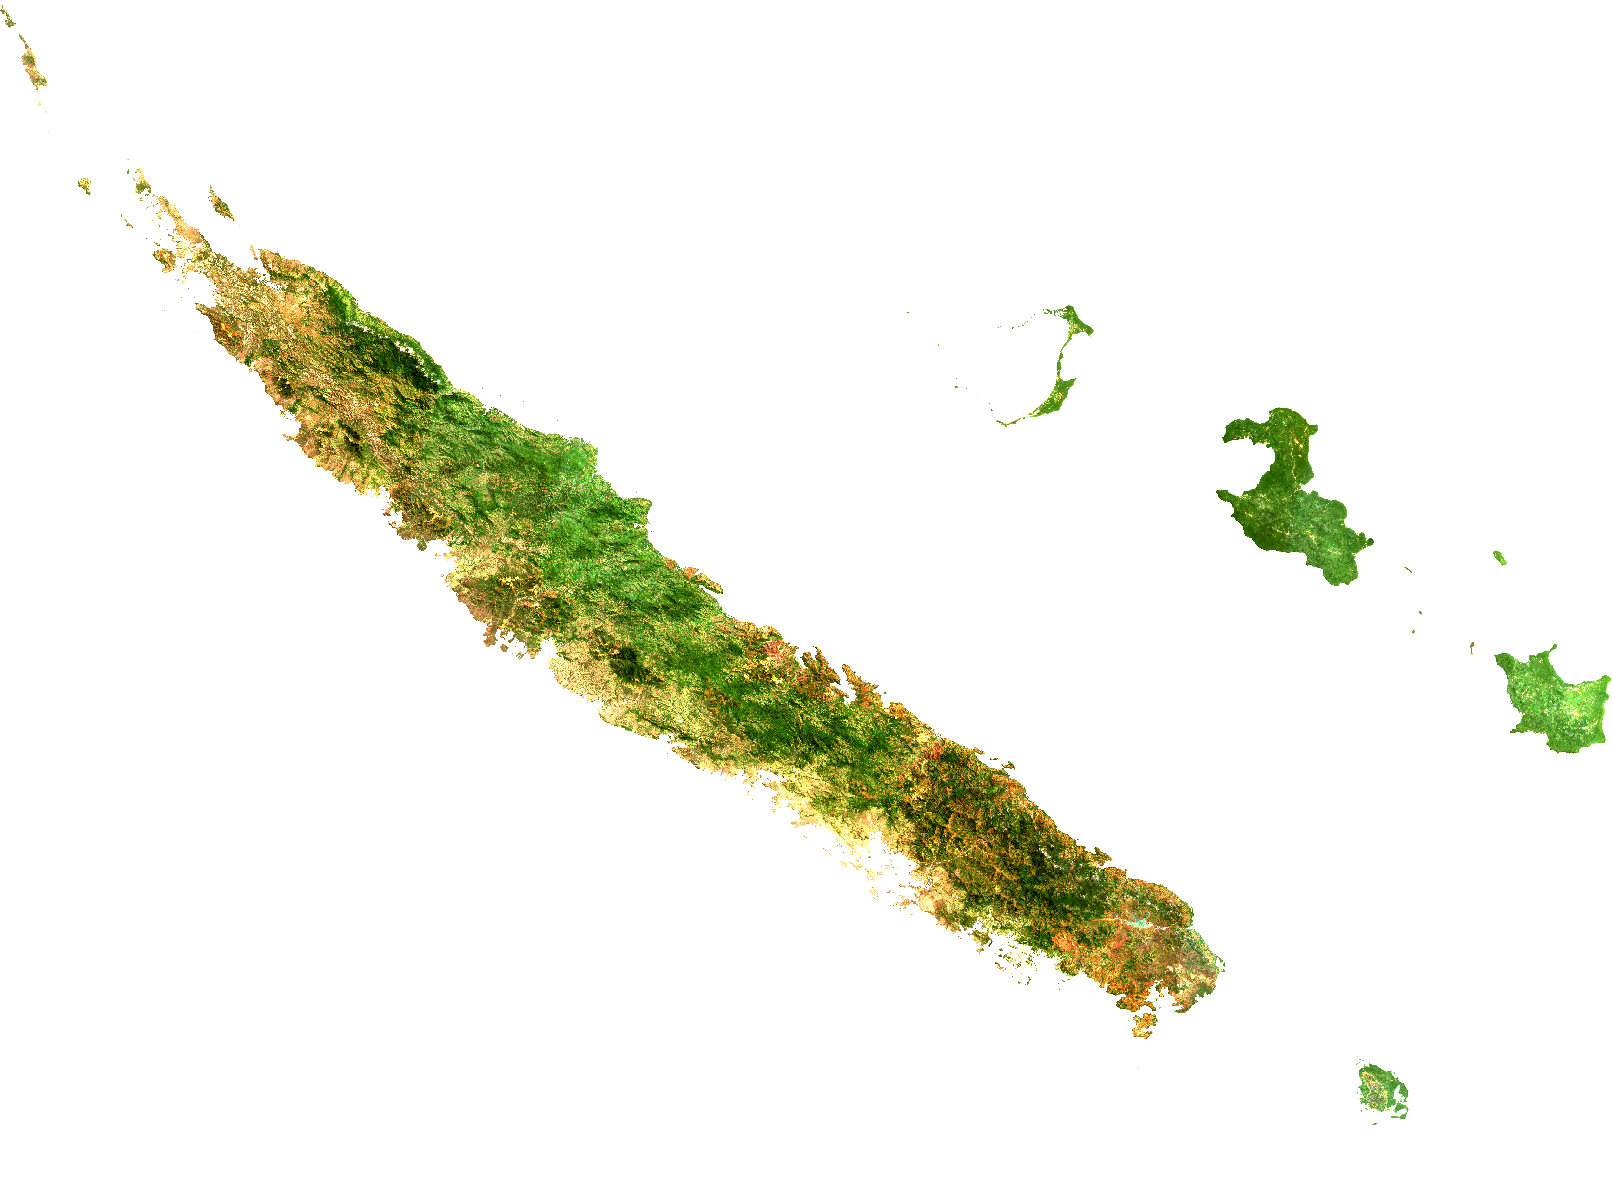
\includegraphics[width=0.5\textwidth]{figs/newcal-S2.png}
\caption{Mosaïque d'images Sentinel-2 couvrant la Nouvelle-Calédonie (2020).}
\end{figure}
\end{frame}

\begin{frame}[label={sec:orgf85887e}]{Emboîtement des données}
\begin{figure}[htbp]
\centering
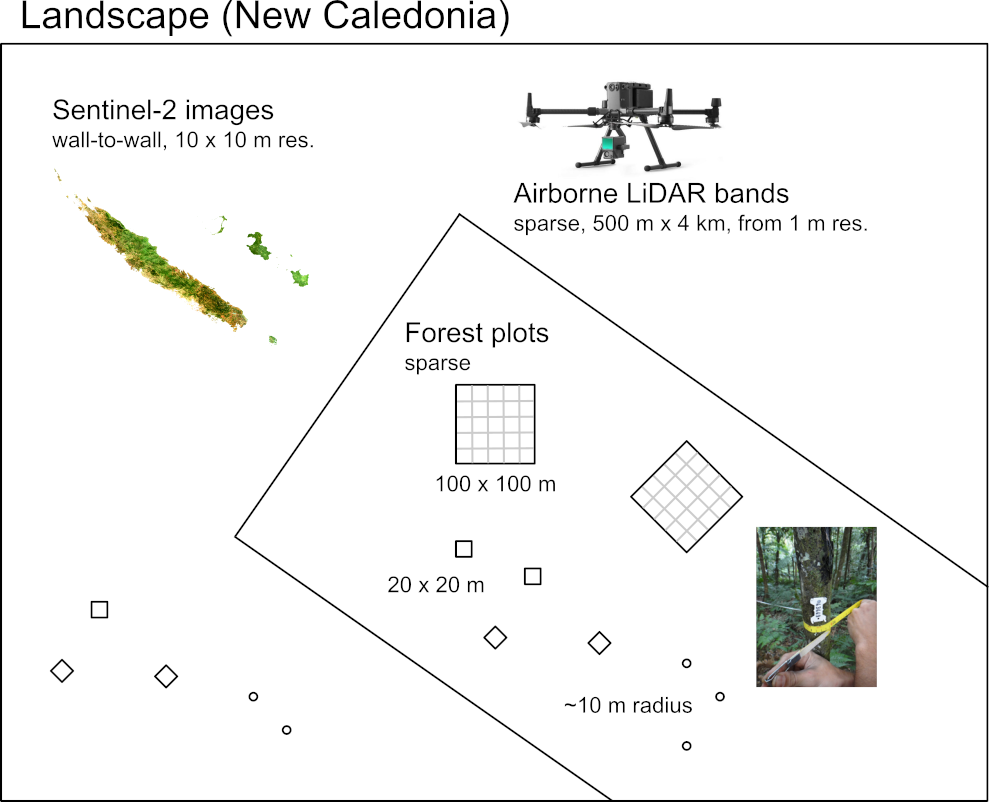
\includegraphics[width=0.7\textwidth]{figs/data-sources.png}
\caption{Emboîtement des différentes données.}
\end{figure}
\end{frame}

\section{Montage de projet}
\label{sec:orgc341204}

\subsection{Institutions partenaires}
\label{sec:org6309663}

\begin{frame}[label={sec:org91e719f}]{Institution partenaires}
\begin{itemize}
\item UMR AMAP:
\begin{itemize}
\item coordinateurs: Ghislain Vieilledent et Thomas Ibanez.
\item participants: équipe d'une dizaine de personnes, spécialités: \\
botanique, LiDAR, télédétection, modélisation statistique, cartographie.
\item localisation: Nouvelle-Calédonie et Montpellier.
\end{itemize}
\item Oeil:
\begin{itemize}
\item participants: Fabien Albouy et Adrien Bertaud.
\item spécialités: étude environnementales, géomatique, communication.
\end{itemize}
\item IAC:
\begin{itemize}
\item participante: Audrey Léopold.
\item spécialités: services écosystémiques, foresterie et biogéochimie.
\end{itemize}
\end{itemize}

\begin{center}

\includegraphics[width=0.5\textwidth]{figs/partners_logos.png}
\end{center}
\end{frame}

\subsection{Calendrier}
\label{sec:org2b2b366}

\begin{frame}[label={sec:org0514f05}]{Calendrier}
\begin{itemize}
\item Projet de 3 ans.
\item 4 workpackages: Inventaires, LiDAR, Cartographie, Coordination.
\end{itemize}

\begin{center}
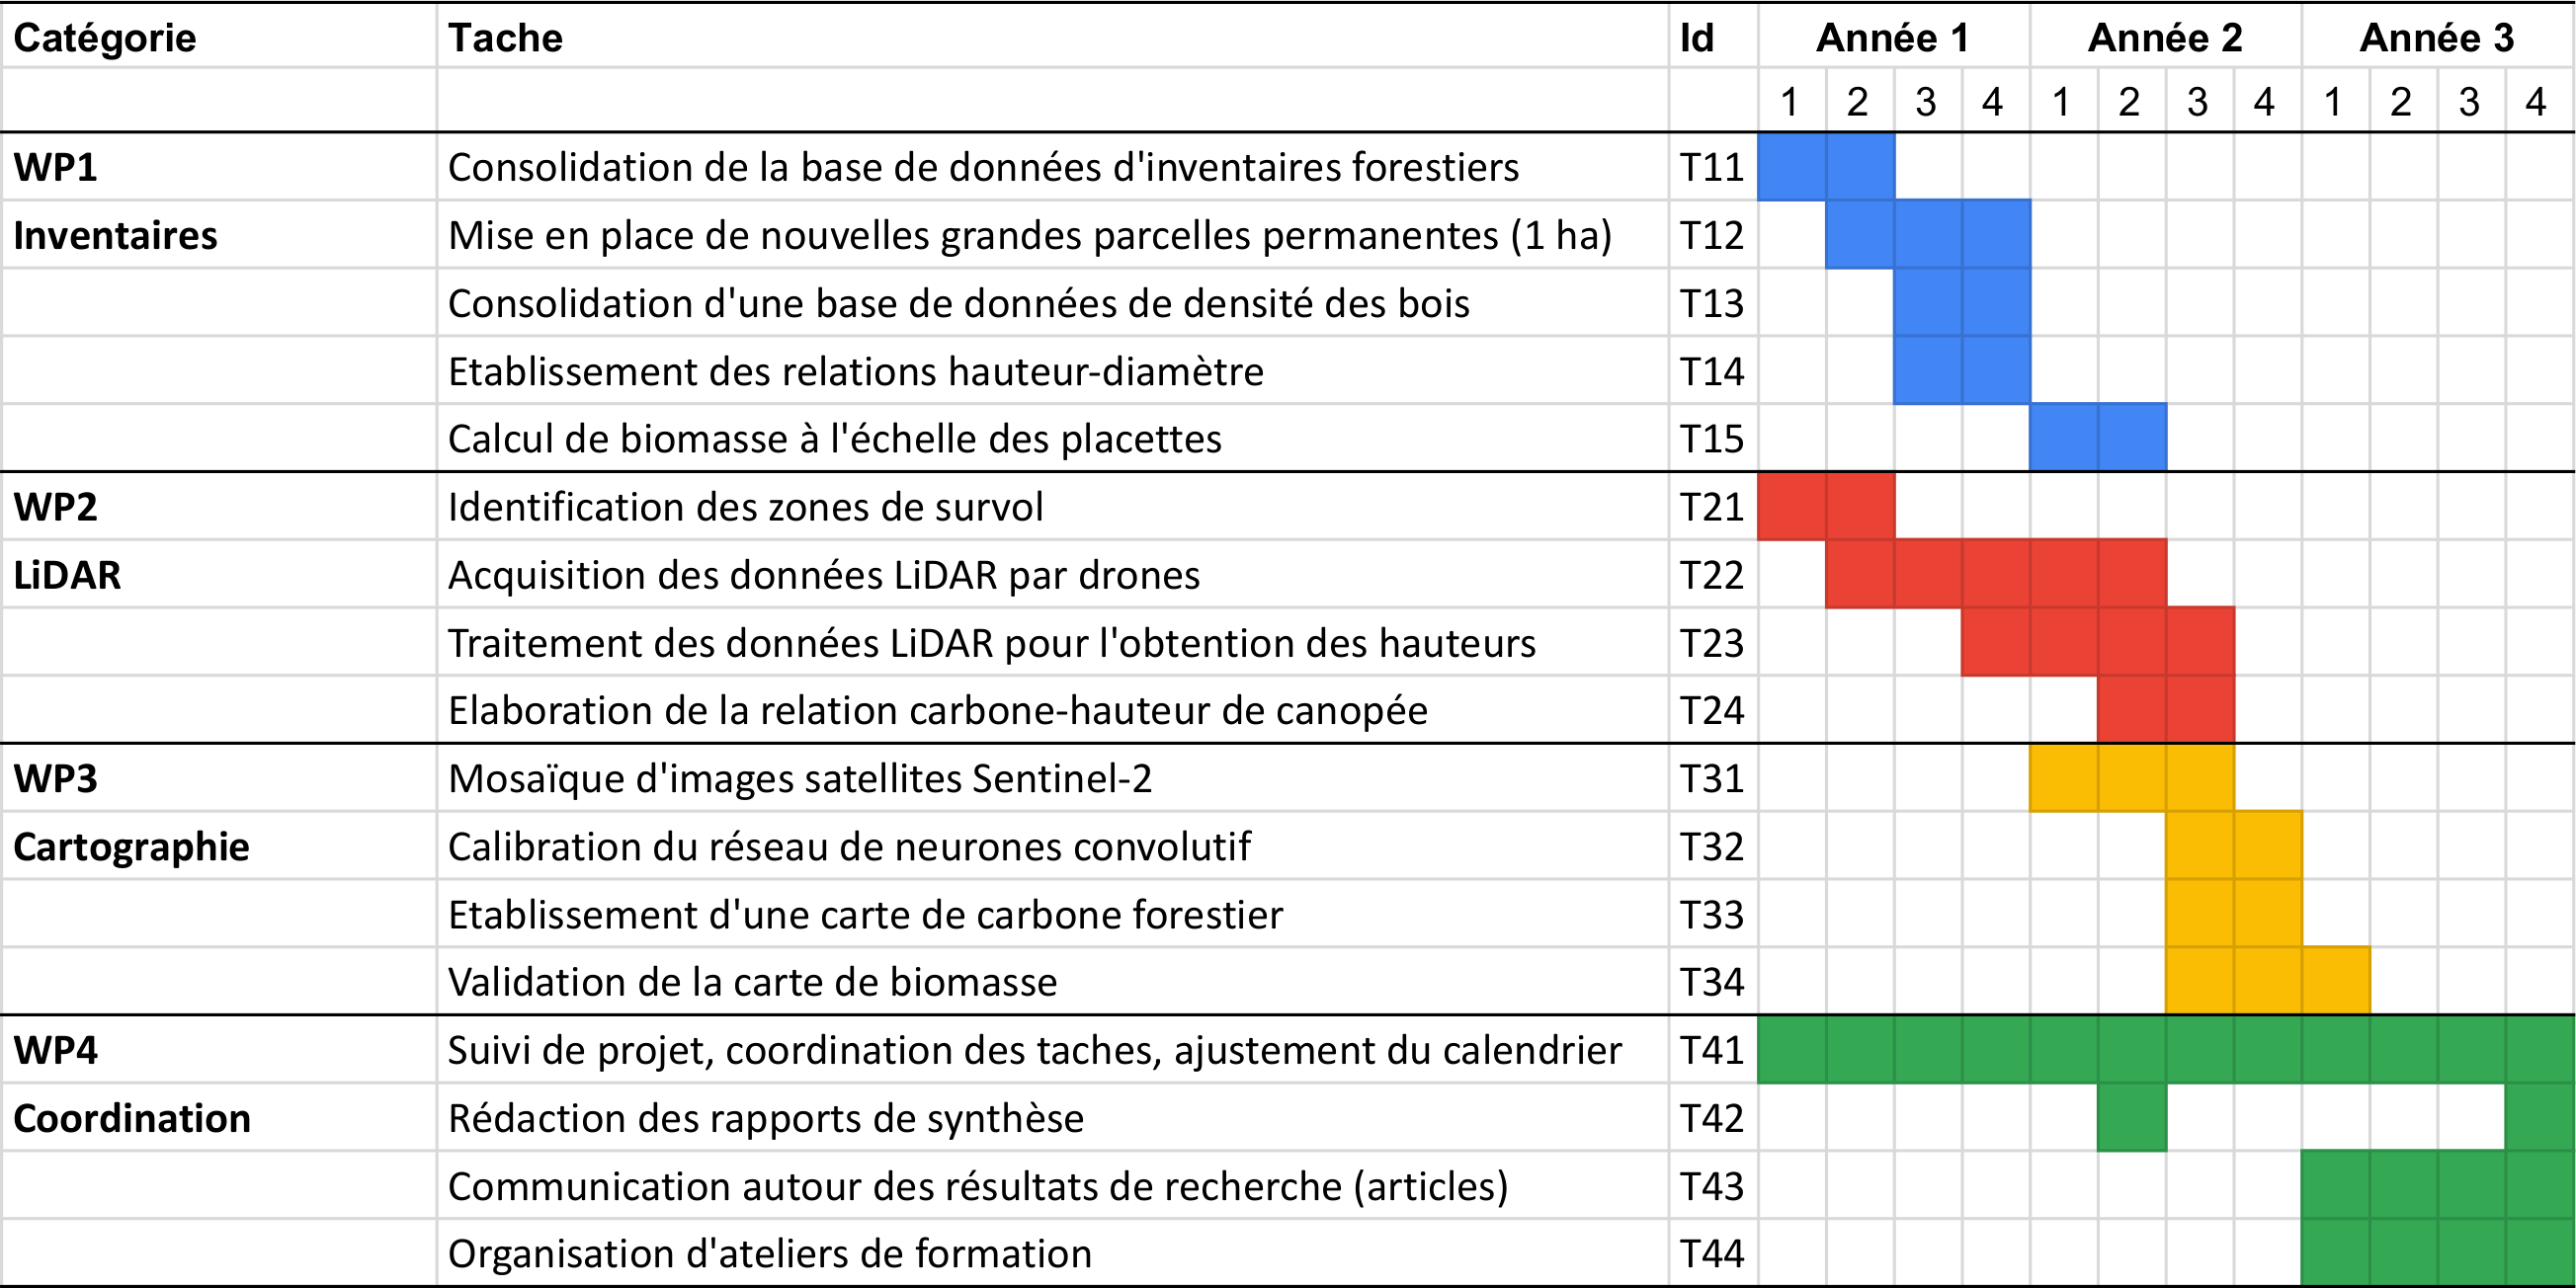
\includegraphics[width=0.9\textwidth]{tabs/diagramme-gantt.png}
\end{center}
\end{frame}

\subsection{Financement}
\label{sec:org6dcac91}

\begin{frame}[label={sec:org69743f7}]{Budget}
\begin{itemize}
\item Budget total estimé: \textasciitilde{}525,000 euros
\item Frais de personnel (15 personnes, 53 mois ETP): 375,000 euros.
\item Frais de fonctionnement (matériels, missions): 150,000 euros.
\end{itemize}

\begin{center}
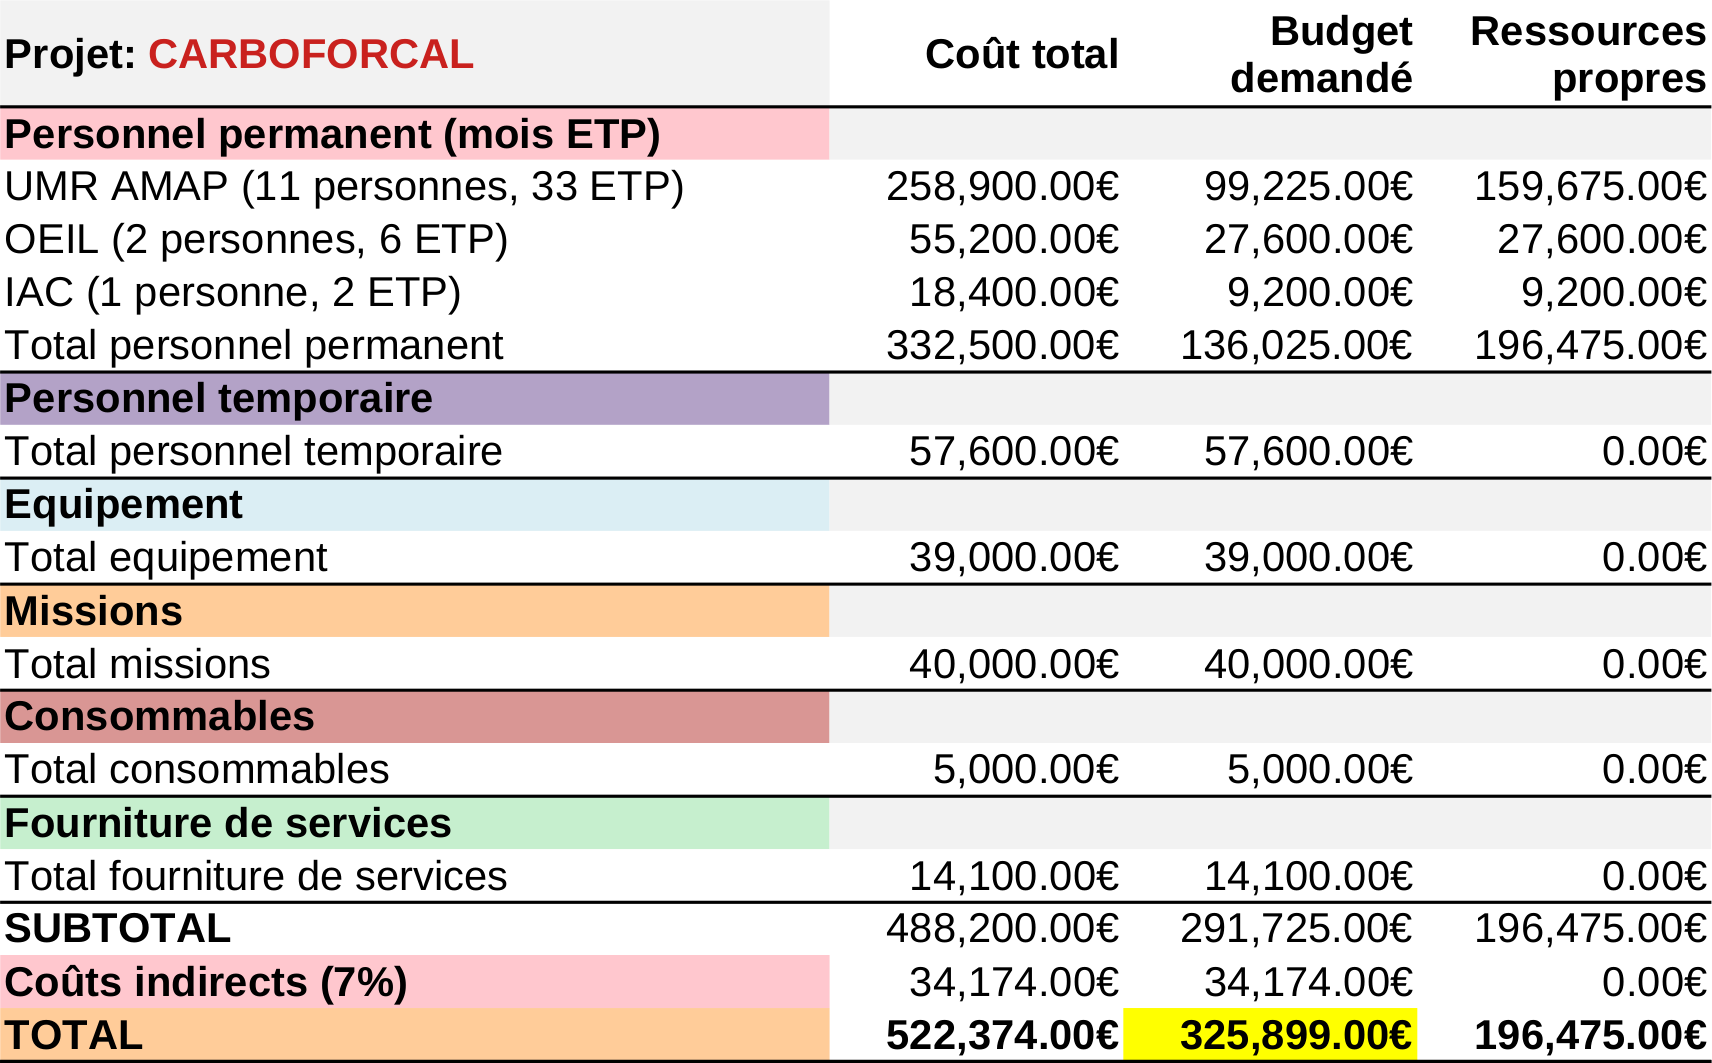
\includegraphics[width=0.7\textwidth]{tabs/budget_Projet.png}
\end{center}
\end{frame}

\begin{frame}[label={sec:orgfa8c2e7}]{Financement}
\begin{itemize}
\item Financement propre: 200,000 euros (> 50\% des frais de personnel).
\item Recherche de financement: 325,000 euros.
\item Co-financements envisageables.
\end{itemize}

\begin{center}
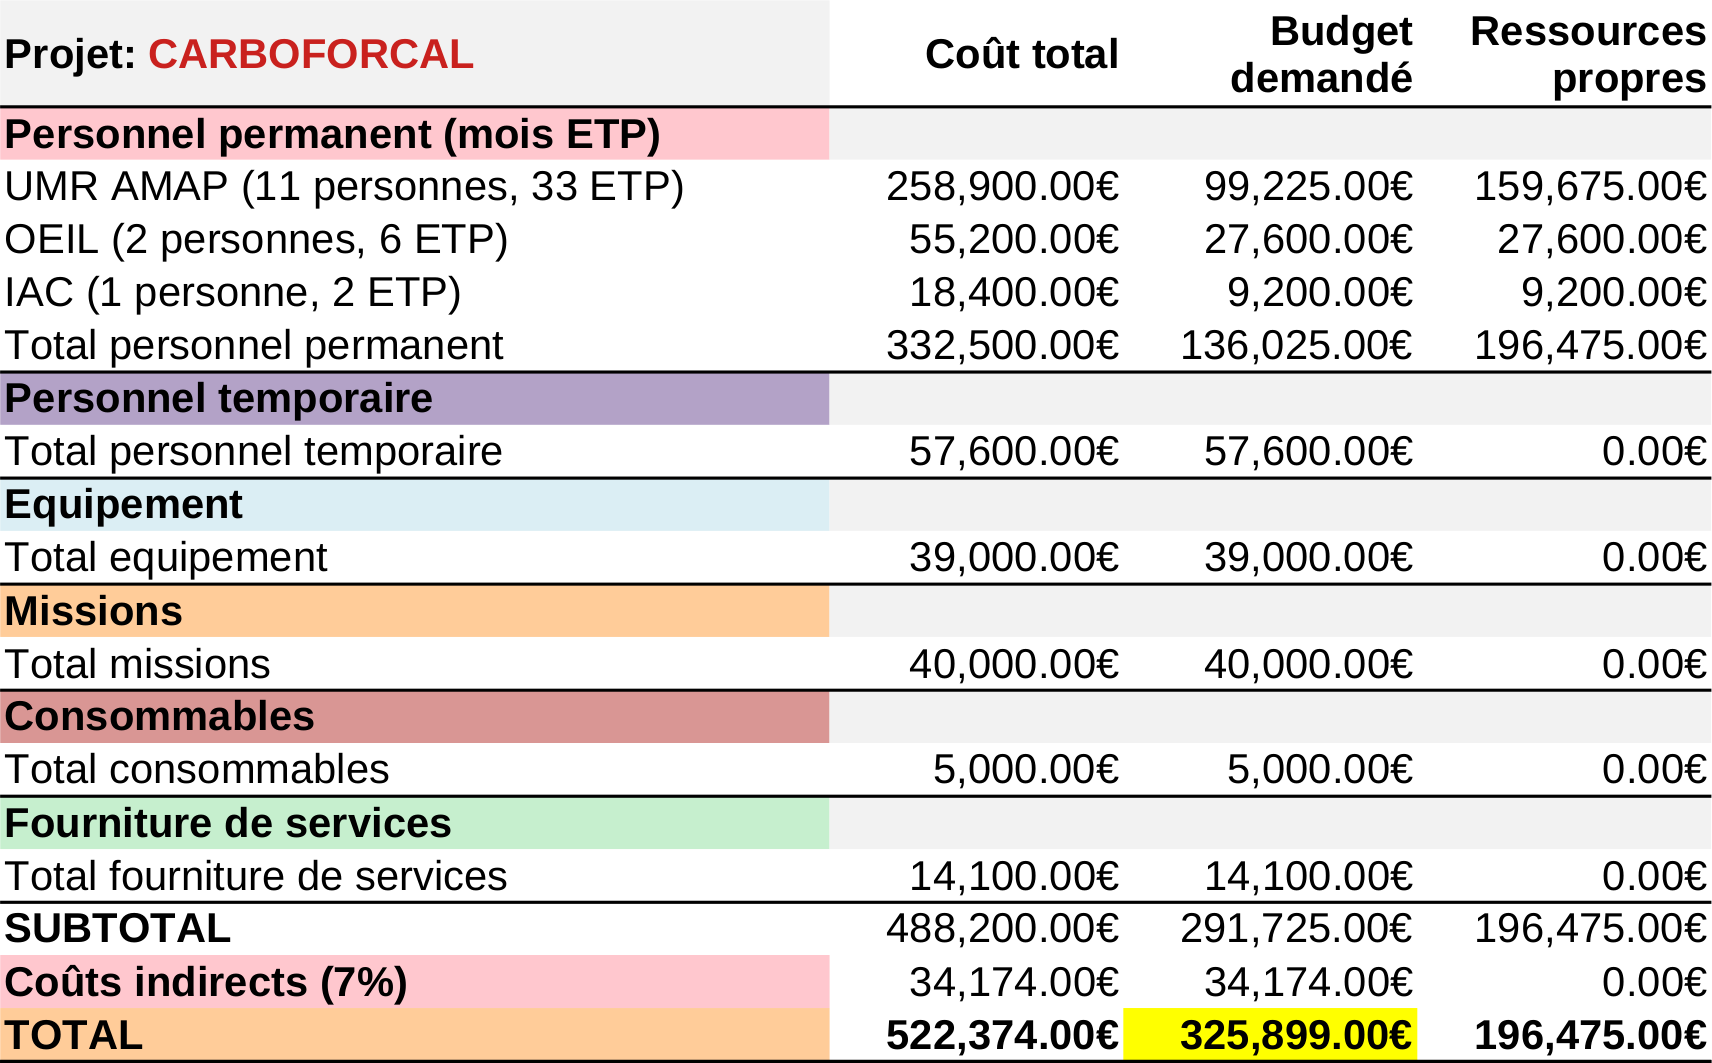
\includegraphics[width=0.7\textwidth]{tabs/budget_Projet.png}
\end{center}
\end{frame}


% %%%%%%%%%%%%%%%%%%%%%%%%%%%%%%%%%%%%%%%%%%%%%%%%%%%%%%%%%%

{
  % Use background image
  \usebackgroundtemplate{%
    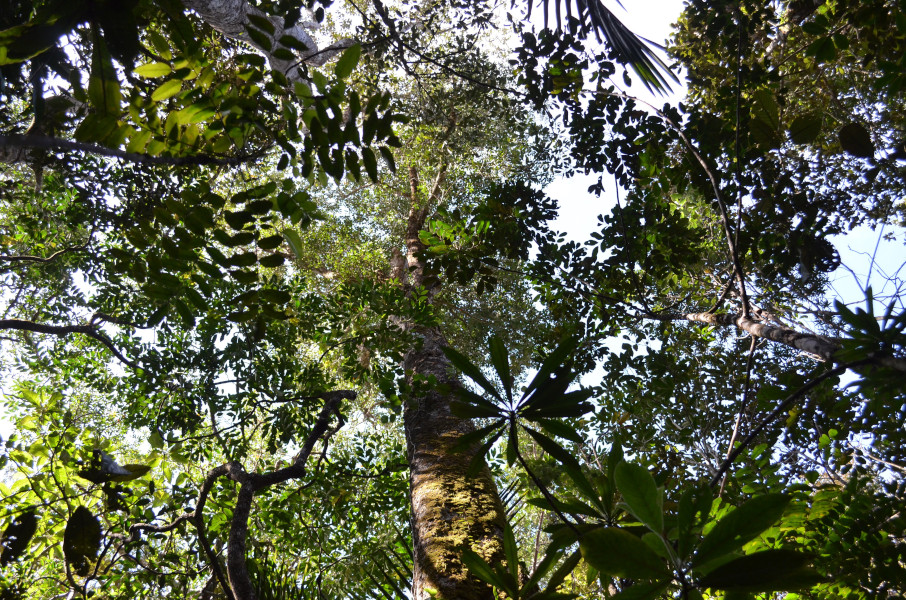
\includegraphics[keepaspectratio=true, height=\paperheight]{figs/Canopy-NC}
  }
  \setbeamertemplate{navigation symbols}{}
  % Remove shadow from block
  \setbeamertemplate{blocks}[rounded][shadow=false]
  \begin{frame}[plain]
  	\vspace*{\stretch{100}} 
    \begin{block}{}
      \begin{center}
        \ldots~Merci pour votre attention~\ldots \\
        \url{https://ecology.ghislainv.fr/presentations} \\
        
\includegraphics[width=0.45\textwidth]{figs/partners_logos}
      \end{center}
    \end{block}
  \end{frame}
}
\end{document}